\documentclass[12pt]{article}

\usepackage[a4paper,  top=1.3in, bottom=1.5in, left=1.5in, right=1.5in]{geometry}

\usepackage[utf8]{inputenc}
\usepackage[T1]{fontenc}
\usepackage{amsmath}
\usepackage{amsfonts}
\usepackage{amssymb}


\usepackage{graphicx, float}
\usepackage{adjustbox}
\graphicspath{{images/}}


%---------------- for graphs ----------------
\usepackage{tikz}
\usepackage{listofitems} % for \readlist to create arrays
\usetikzlibrary{arrows.meta} % for arrow size
\usepackage[outline]{contour} % glow around text
\contourlength{1.4pt}

% COLORS
\usepackage{xcolor}
\colorlet{myred}{red!80!black}
\colorlet{myblue}{blue!80!black}
\colorlet{mygreen}{green!60!black}
\colorlet{myorange}{orange!70!red!60!black}
\colorlet{mydarkred}{red!30!black}
\colorlet{mydarkblue}{blue!40!black}
\colorlet{mydarkgreen}{green!30!black}

% STYLES
\tikzset{
  >=latex, % for default LaTeX arrow head
  node/.style={thick,circle,draw=myblue,minimum size=22,inner sep=0.5,outer sep=0.6},
  node in/.style={node,green!20!black,draw=mygreen!30!black,fill=mygreen!25},
  node hidden/.style={node,blue!20!black,draw=myblue!30!black,fill=myblue!20},
  node convol/.style={node,orange!20!black,draw=myorange!30!black,fill=myorange!20},
  node out/.style={node,red!20!black,draw=myred!30!black,fill=myred!20},
  connect/.style={thick,mydarkblue}, %,line cap=round
  connect arrow/.style={-{Latex[length=4,width=3.5]},thick,mydarkblue,shorten <=0.5,shorten >=1},
  node 1/.style={node in}, % node styles, numbered for easy mapping with \nstyle
  node 2/.style={node hidden},
  node 3/.style={node out}
}
\def\nstyle{int(\lay<\Nnodlen?min(2,\lay):3)} % map layer number onto 1, 2, or 3


\tikzset{basic/.style={draw,fill=none,
                       text badly centered,minimum width=3em}}
\tikzset{input/.style={basic,circle,minimum width=3.5em}}
\tikzset{weights/.style={basic,rectangle,minimum width=2em}}
\tikzset{functions/.style={basic,circle, minimum width=4em}}
\newcommand{\addaxes}{\draw (0em,1em) -- (0em,-1em)
                            (-1em,0em) -- (1em,0em);}
\newcommand{\relu}{\draw[line width=1.5pt] (-1em,0) -- (0,0)
                                (0,0) -- (0.75em,0.75em);}
\newcommand{\stepfunc}{\draw[line width=1.5pt] (0.65em,0.65em) -- (0,0.65em) 
                                    -- (0,-0.65em) -- (-0.65em,-0.65em);}


%-----------------------------------------------------


\renewcommand{\figurename}{Slika}



\renewcommand{\baselinestretch}{1.2} % Line spacing

% Parskip and parindent
\setlength{\parindent}{0pt} % Begin of paragraph indentation
\setlength{\parskip}{1em} % Paragraph spacing

%--- for references ---------
\usepackage[
   backend=biber,
   style=numeric
   ]{biblatex}

\addbibresource{bibliography.bib}
\AtBeginBibliography{\vspace*{10pt}}
%----------------------------

\begin{document}

   % Title Page
   \newgeometry{top=1in, bottom=1in, left=1in, right=1in} % New margins for title page
   \begin{titlepage}
      \begin{center}
         
         % add your university logo here
         % negative value moves the logo up
         \vspace*{-1in}
         
\includegraphics[width=0.4\textwidth]{raf_logo.png}

         % set font size to 14pt
         \vspace{1in}
         \Large
         \textbf{DIPLOMSKI RAD}
         
         % set horizontal margin for the title to 1.5in and center it
         \vspace{1in}
         \Huge
         \textbf{Slika je vredna 16x16 reči: \\ Vision Transformeri}
         
         \vspace{1in}


         \fontsize{14pt}{18pt}\selectfont
         \textbf{Vanja Kovinić} \\
         \textbf{RN 42/2020}
         \vspace*{1.5in}
         
         \begin{center}
            \normalsize
            \begin{tabular}{p{0.7\textwidth} p{0.5\textwidth}}
               \fontsize{14pt}{18pt}\selectfont   
               \textbf{Mentor:} & 
            
               \fontsize{14pt}{18pt}\selectfont
               \textbf{Komisija:} \\
               dr Nemanja Ilić & dr Nemanja Ilić \\
                                 & dr Nevena Marić \\
            \end{tabular}
         \end{center}

         \vspace*{\fill}

         \normalsize
         Beograd, septembar 2024.


         
      \end{center}
   \end{titlepage}
   \restoregeometry % Restore original margins

   \newpage


   % Table of Contents
   \thispagestyle{empty} % Remove page number from Abstract page
   \renewcommand{\contentsname}{Sadržaj}
   \tableofcontents

   
   \newpage
   
   \thispagestyle{empty} % Remove page number from Abstract page

   % Define a command to format a specific section title
   \newcommand{\specialsection}[1]{
      \section*{\centering{#1}} % Center and italicize the section title
   }

   \vspace*{0.5in}
   \specialsection{Apstrakt}
   

   \vspace*{0.5in}

   Ovaj diplomski rad istražuje \textbf{Vision Transformere} (\textbf{ViT}),
   nov pristup u oblasti računarskog vida koji koristi arhitekturu
   transformera prvobitno razvijenu za obradu prirodnog jezika. Prvi deo rada pruža detaljan pregled arhitekture transformera, 
   uključujući ključne komponente kao što su \textbf{\textit{self-attention} mehanizam} i \textbf{poziciono enkodovanje},
   i diskutuje njihove svrhe i funkcionalnosti. Nakon toga, fokus se prebacuje
   na Vision Transformere, objašnjavajući kako se slike transformišu
   u \textbf{tokene} i obrađuju kroz \textbf{enkoder transformera} kako bi se primenili na rešavanje vizuelnih zadataka.

   Rad zatim ulazi u praktične aspekte implementacije Vision Transformera,
   uključujući izbor i podešavanje \textbf{hiperparametara} za poboljšanje performansi.
   Izvršeno je i poređenje sa referentnim implementacijama, i predložen pristup za 
   poboljšanje performansi. Prikazani su različiti
   eksperimenti, zajedno sa diskusijom njihovih rezultata, pružajući uvid
   u efikasnost i izazove povezane sa Vision Transformerima.

   Na kraju, rad naglašava značaj Vision Transformera u oblasti računarskog vida, 
   prikazujući njihov potencijal i ograničenja, kao i njihove praktične primene.

   \newpage
   \pagenumbering{arabic}
   \setcounter{page}{1}

   \section{Uvod}
   
   \textit{"Pre otprilike 540 miliona godina, 
   Zemlja je bila obavijena tamom.
   Ovo nije bilo zbog nedostatka svetlosti,
   već zato što organizmi još uvek nisu razvili sposobnost da vide.
   Iako je sunčeva svetlost mogla da prodre u okeane do dubine
   od 1.000 metara i hidrotermalni izvori na dnu mora isijavali 
   svetlost u kojoj je život cvetao, nijedno oko nije se moglo naći 
   u tim drevnim okeanima, nijedna retina, rožnjača ili sočivo. 
   Sva svetlost i život nikada nisu viđeni. Koncept gledanja nije ni postojao tada 
   i ova sposobnost nije ostvarena sve dok nije stvorena.
   }
   
   \textit{Iz nama nepoznatih razloga, trilobiti su se pojavili kao prva bića sposobna
   da spoznaju svetlost. Oni su prvi prepoznali da postoji nešto izvan
   njih samih, svet okružen višestrukim jedinkama. Rađenje vida se smatra da je pokrenulo
   kambrijsku eksploziju, period u kojem se veliki broj vrsta životinja pojavljuje u 
   fosilnom zapisu. Vid je započeo kao pasivno iskustvo, jednostavno propuštanje svetlosti, 
   ali je ubrzo postao aktivniji. Nervni sistem je počeo da evoluira, vid je prešao u uvid, 
   gledanje je postalo razumevanje, a razumevanje je dovelo do akcije, a sve to je dovelo do 
   nastanka inteligencije.}
   
   \textit{Danas nismo više zadovoljni vizuelnom spoznajom koju nam je priroda dala. 
   Radoznalost nas je navela da stvorimo mašine koje mogu da "vide" kao mi, pa čak i inteligentnije."} - Li Fei-Fei \cite{li_fei_fei}
   

   \subsection{Istorija i motivacija}
   \vspace{-0.5cm}
   \subsubsection{Rani Razvoj u Računarskom Vidu}

   Koreni računarskog vida potiču iz ranih pokušaja da se razume 
   i interpretira vizuelni podatak korišćenjem matematičkih modela i računara. 
   U početku, istraživanja u oblasti računarskog vida fokusirala su se na 
   jednostavne zadatke kao što su detekcija ivica, prepoznavanje objekata i 
   osnovna obrada slika. Rane metode su se u velikoj meri oslanjale na ručnu 
   izradu karakteristika (engl. \textbf{\textit{features}}) slike i algoritme dizajnirane da imitiraju osnovne aspekte 
   ljudskog vida.

   \subsubsection{Uspon Dubokog Učenja}

   Značajan preokret u računarskom vidu dogodio se sa pojavom \textbf{dubokog učenja}. 
   \textbf{Konvolucione Neuronske Mreže} (\textbf{CNNs}), koje su predstavili Yann LeCun i drugi \cite{lecun_cnn} 
   krajem 1980-ih i početkom 1990-ih, revolucionisale su ovu oblast uvođenjem automatskog 
   ekstraktovanja karakteristika kroz slojeve koji se uče (engl. \textbf{\textit{learnable features}}). \textbf{CNN}-ovi su pokazali izuzetne 
   performanse u različitim zadacima klasifikacije slika, omogućavajući računarima da 
   nauče složene reprezentacije vizuelnih podataka. Ovo otkriće je kasnije propaćeno uspehom modela 
   kao što su \textbf{AlexNet} \cite{alexnet}, \textbf{VGGNet} \cite{vgg} i \textbf{ResNet} \cite{resnet}, koji su postavili nove standarde u izazovima 
   prepoznavanja slika.

   \subsubsection{Ograničenja CNN-ova}

   Uprkos svom uspehu, \textbf{CNN}-ovi imaju inherentna ograničenja 
   koja su motivisala potragu za novim pristupima. Jedan od 
   značajnih nedostataka je njihova poteškoća u povezivanju udaljenih zavisnosti
   i globalnog konteksta unutar slike. \textbf{CNN}-ovi obično obrađuju slike kroz seriju 
   lokalizovanih konvolucionih operacija, što može ograničiti njihovu sposobnost da 
   razumeju odnose između udaljenih elemenata na slici.

   \subsubsection{Motivacija za uvođenje Vision Transformera}

   Pojava \textbf{Vision Transformera} (\textbf{ViT}) predstavlja odgovor na ova ograničenja. 
   Inspirisani uspehom modela transformera u obradi prirodnog jezika (\textbf{NLP}), 
   istraživači su pokušali da primene iste principe u računarskom vidu. 
   Transformeri koriste \textbf{\textit{self-attention}} mehanizam za povezivanje globalnih zavisnosti, 
   što ih čini pogodnim za zadatke koji zahtevaju razumevanje 
   složenih odnosa unutar vizuelnih podataka.
   
   \newpage

   \textbf{Vision Transformeri} rešavaju nekoliko izazova sa kojima se suočavaju \textbf{CNN}-ovi. 
   Pretvaranjem slika u sekvence parčića (engl. \textbf{\textit{image patches}}) i primenom \textbf{\textit{self-attention}} mehanizma preuzetim iz \textbf{transformera}, 
   \textbf{ViT}-ovima mogu efikasnije modelovati globalni kontekst. 
   Ovaj pristup omogućava \textbf{ViT}-ovima da postignu vrhunske performanse na različitim  
   testovima klasifikacije slika i pokazuje njihov potencijal da unaprede oblast računarskog vida.

   \subsection{Konvolucione Neuronske Mreže (\textbf{CNN})}
   \subsubsection{Istorija \textbf{CNN}-ova}
   Konvolucione neuronske mreže su razvijene 
   i prvi put korišćene oko 1980-ih. Tokom tog perioda, primarna primena 
   \textbf{CNN}-ova bila je prepoznavanje rukom pisanih cifara, što je našlo 
   praktičnu primenu u poštanskom sektoru za čitanje poštanskih i PIN kodova. 
   Rani modeli \textbf{CNN}-ova, kao što je \textbf{LeNet} \cite{lenet} koji je razvio Yann LeCun, pokazali su 
   potencijal CNN-ova za zadatke prepoznavanja cifara.

   Međutim, šira primena \textbf{CNN}-ova bila je ograničena značajnim izazovima. 
   Duboki modeli učenja, uključujući \textbf{CNN}-ove, zahtevaju ogromne količine 
   podataka za obuku i značajne računarske resurse, koji u to vreme nisu 
   bili lako dostupni. Pored toga, \textbf{\textit{backpropagation}} algoritam, 
   koji je neophodan za obuku neuronskih mreža, bio je računarski skup. 
   Ova ograničenja su ograničila upotrebu \textbf{CNN}-ova uglavnom na poštanski sektor, 
   i tehnologija nije uspela da stekne širu primenu u oblasti mašinskog učenja.

   Oživljavanje \textbf{CNN}-ova došlo je 2012. godine, kada su Alex Krizhevsky, zajedno 
   sa Ilyom Sutskeverom i Geoffreyjem Hintonom, prepoznali potencijal dubokog 
   učenja sa višeslojnim neuronskim mrežama. Ovo oživljavanje je pokrenuto nekoliko 
   ključnih faktora: dostupnost velikih skupova podataka, kao što je \textbf{\textit{ImageNet}} \cite{imagenet} skup sa 
   milionima označenih slika, i značajna unapređenja u računarskim resursima, posebno \textbf{GPU}-ovima 
   (engl. \textbf{\textit{graphics processing unit}}). Ovi razvojni događaji omogućili su istraživačima da prevaziđu prethodna ograničenja i u 
   potpunosti iskoriste mogućnosti konvolucionih neuronskih mreža.

   \subsubsection{Ljudski vizuelni sistem kao inspiracija}
   Arhitektura konvolucionih neuronskih mreža je analogna načinu na koji su neuroni u
   ljudskom mozgu povezani i inspirisana je organizacijom \textbf{vizuelnog korteksa}. 
   Pojedinačni neuroni reaguju na stimuluse samo u ograničenom delu vizuelnog polja 
   poznatom kao \textbf{receptivno polje} (engl. \textbf{\textit{receptive field}}). 
   Ova polja se preklapaju kako bi se pokrilo čitavo vizuelno područje.


   \begin{figure}[h!]
      \centering
      \vspace{1.5cm} % Add vertical space
      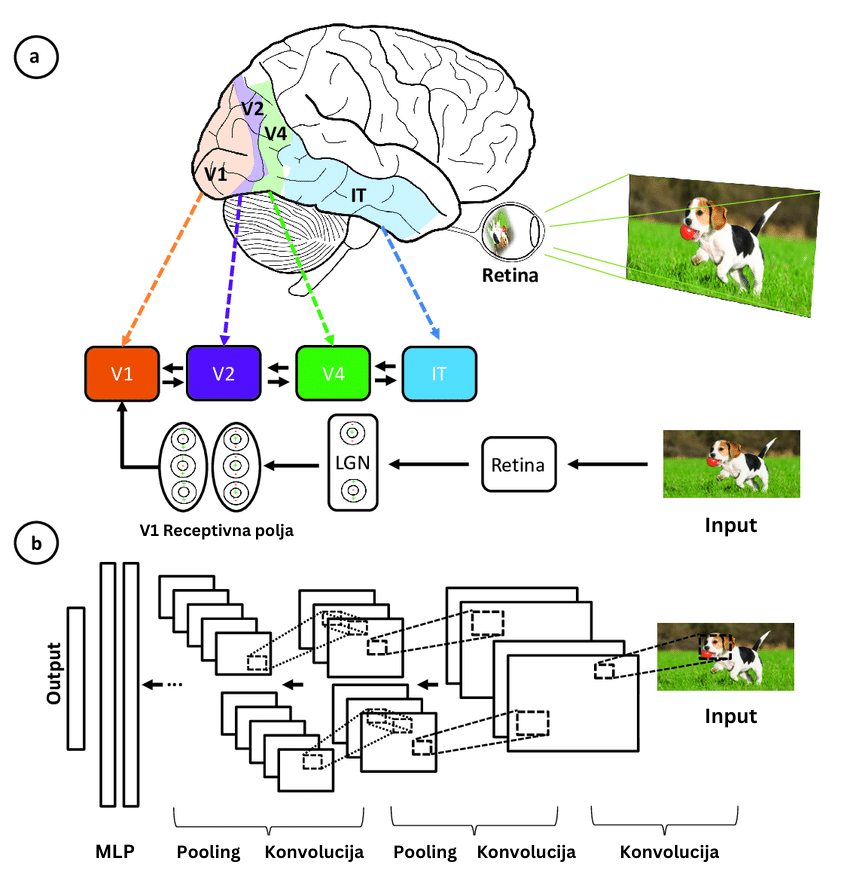
\includegraphics[width=0.8\textwidth]{visual_cortex.png}
      \caption{Paralela između organizacije vizuelnog korteksa i \textbf{CNN} arhitekture}
      \label{fig:visual_cortex}
   \end{figure}

   \newpage

   Glavne sličnosti \cite{human_visual_cortex} između organizacije vizuelnog korteksa i arhitekture \textbf{CNN}-ova su:
   \begin{itemize}
   \item \textbf{Hijerarhijska arhitektura}: I \textbf{CNN} i vizuelni korteks imaju hijerarhijsku strukturu, 
   gde se jednostavni oblici izvlače u početnim slojevima, a složeniji oblici se grade u dubljim slojevima. 
   Ovo omogućava kompleksniju reprezentaciju vizuelnog inputa.
   \item \textbf{Lokalna povezanost}: Neuroni u vizuelnom korteksu su povezani samo sa 
   lokalnim regionom inputa, a ne sa celim vizuelnim poljem. Slično tome, neuroni 
   u sloju \textbf{CNN}-a su povezani samo sa lokalnim regionom inputa putem \textbf{konvolucione operacije}. 
   Ova lokalna povezanost omogućava efikasnost.
   \item \textbf{Translaciona invarijantnost}: Neuroni vizuelnog korteksa mogu detektovati karakteristike
    bez obzira na njihovu lokaciju u vizuelnom polju. \textbf{\textit{Pooling}} slojevi u \textbf{CNN}-u pružaju određeni 
    stepen \textbf{translacione invarijantnosti}.
    \item \textbf{Višestruke \textit{feature} mape}: Na svakoj fazi vizuelne obrade, izvlače se različite \textbf{\textit{feature}} mape.
    \textbf{CNN}-ovi ovo imitiraju putem višestrukih jezgara (engl. \textbf{\textit{kernels}}) koji detektuju različite karakteristike
      u svakom konvolucionom sloju.
   \item \textbf{Nelinearnost}: Neuroni u vizuelnom korteksu pokazuju osobine nelinearnosti. 
   \textbf{CNN}-ovi postižu nelinearnost putem \textbf{aktivacionih funkcija}, koje se primenjuju nakon svake konvolucije.
   
   \end{itemize}
   
   \newpage

   \subsubsection{Arhitektura \textbf{CNN}-ova}
   Arhitektura \textbf{CNN}-a biće prikazana na primeru klasifikacionog
    problema\footnote{Gradivni elementi CNN-a su identični, bez obzira na to
     da li je u pitanju problem regresije ili druge prirode; jedina razlika leži u MLP sloju}, 
     gde je cilj modela da klasifikuje slike u jednu od $P$ klasa, kao što je prikazano na slici 2.


     \begin{figure}[h!]
      \centering
      \adjustbox{scale=0.45,center}{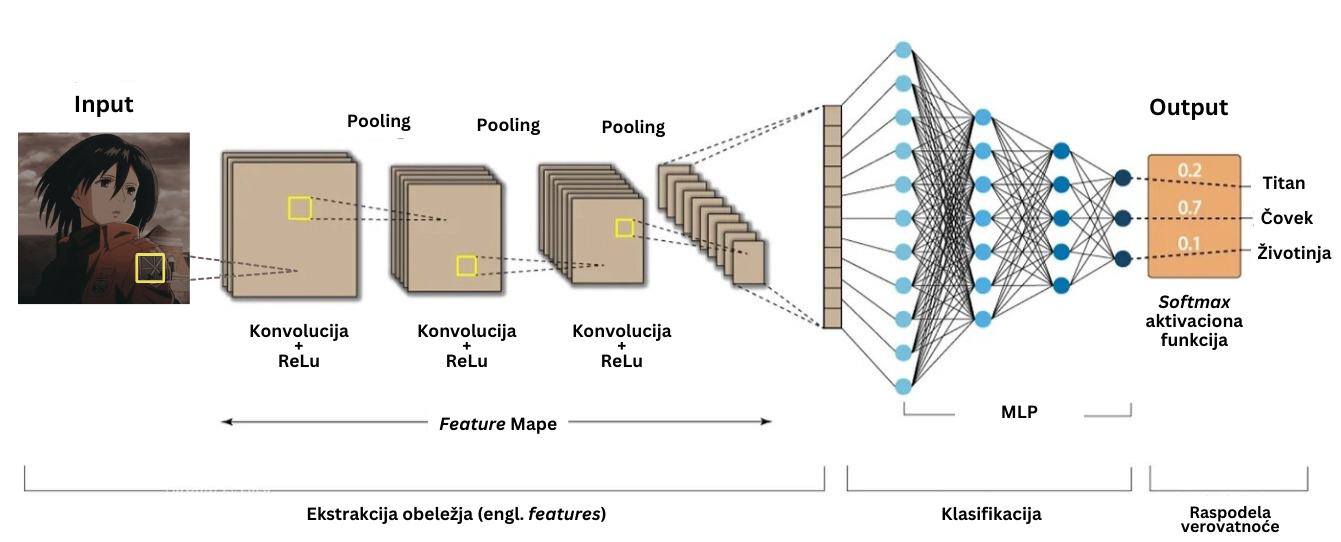
\includegraphics{cnn_arhitecture.png}} % Adjust the scale factor as needed
      \caption{Primer arhitekture \textbf{CNN}-a za klasifikaciju slika}
      \label{fig:cnn_architecture}
    \end{figure}
    
    \vspace{0.7cm}
   
    Sastavni deo \textbf{CNN}-a su:
    \begin{itemize}
      % remove white space between first item and start of the list
      \vspace{-0.5cm}
      \setlength\itemsep{0em}
      \item \textbf{Konvolucioni slojevi}
      \item \textbf{\textit{Pooling} slojevi}
      \item \textbf{Višeslojni perceptron (engl. \textbf{\textit{Multi-Layer Perceptron}} - \textbf{MLP})}
   \end{itemize}

   \newpage

   \subsection*{Konvolucioni slojevi}
   \subsubsection*{1. Konvoluciona operacija}
   U \textbf{konvolucionom sloju}, osnovna operacija je \textbf{konvolucija} ulazne slike sa \textbf{kernelom} (poznatim i kao \textbf{filter}).
   Cilj ove operacije je detektovanje karakteristika kao što su ivice, teksture 
   ili šare u ulaznim podacima.

   Neka je ulazna slika predstavljena kao 2D matrica \( I \) 
   sa dimenzijama \( H \times W \), gde je \( H \) visina, 
   a \( W \) širina slike (pogledati sliku 3). Neka je \( K \) 2D kernel sa 
   dimenzijama \( f \times f \), gde je \( f \) veličina kernela.
   
   Konvolucija operacija se može matematički izraziti kao:
   \[
   S(i, j) = \sum_{m=0}^{f-1} \sum_{n=0}^{f-1} I(i+m, j+n) \cdot K(m, n)
   \]
   gde \( S(i, j) \) predstavlja vrednost izlazne \textbf{\textit{feature}} mape na poziciji 
   \((i, j)\). Ovde, \( (i, j) \) označava poziciju na ulaznoj slici gde se primenjuje kernel.

   \subsubsection*{2. Izlaz konvolucione operacije}
   Rezultat primene kernela na ulaznu sliku je \textit{feature} mapa \( F \) 
   sa dimenzijama \((H - f + 1) \times (W - f + 1)\), pod pretpostavkom da se ne 
   koristi \textit{padding}. Veličina \textit{feature} mape je 
   smanjena u odnosu na ulaznu sliku zbog klizne operacije kernela.

   \newpage   

   \begin{figure}[h!]
      \centering
      \adjustbox{scale=0.2,center}{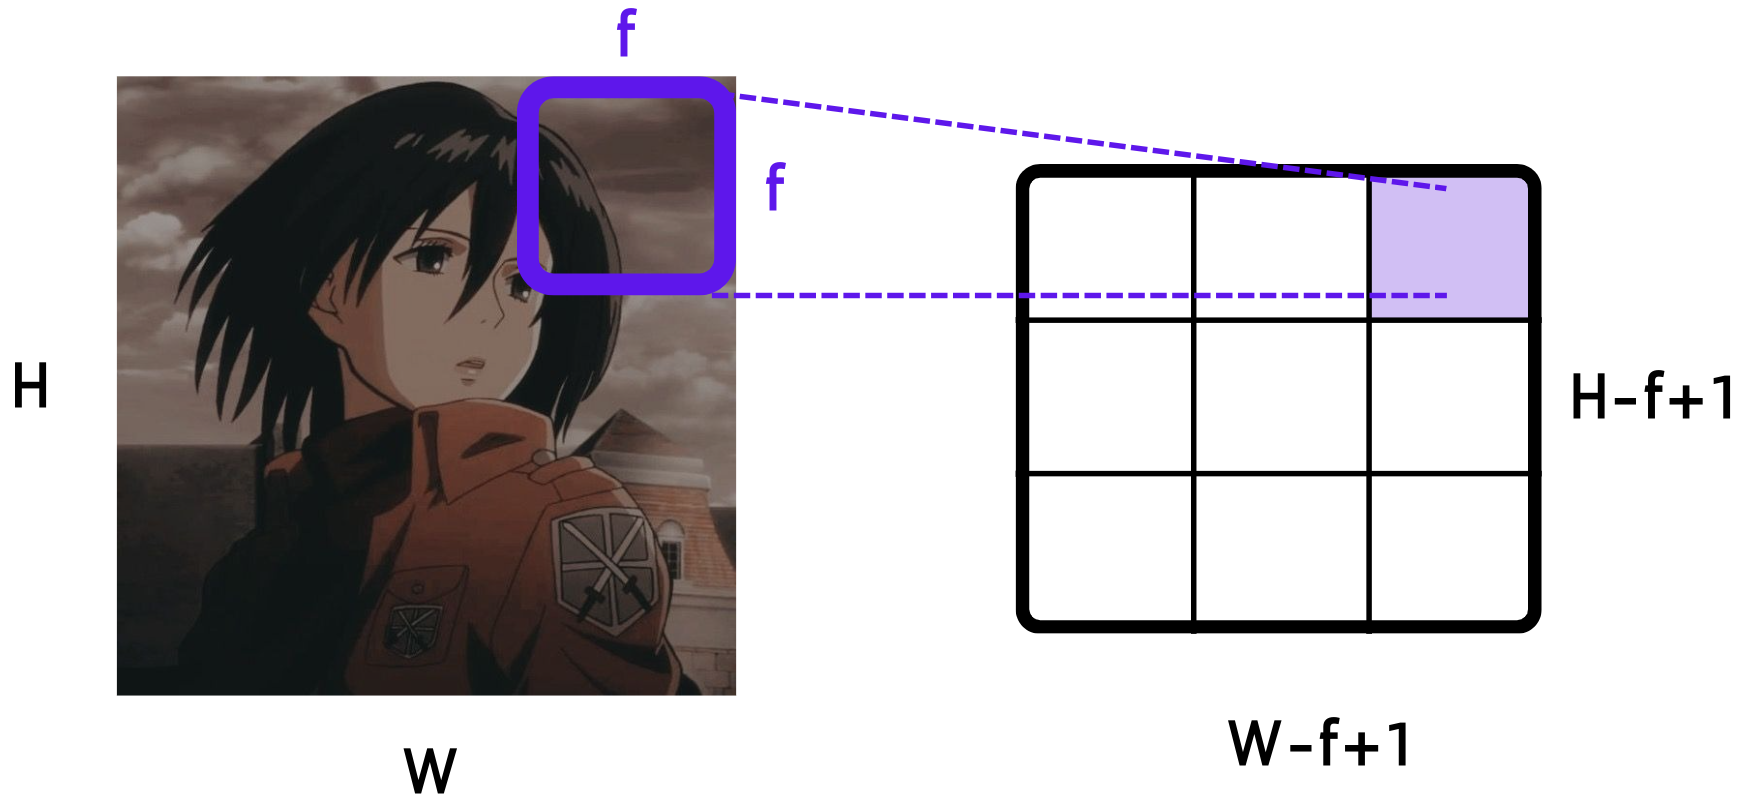
\includegraphics{convolution.png}} % Adjust the scale factor as needed
      \caption{Dimenzije ulazne slike i \textit{feature} mape u jednom konvolucionom sloju}
      \label{fig:convolution}
    \end{figure}

    \subsubsection*{3. Popunjavanje (engl. Padding)}

    Popunjavanje se koristi za kontrolu prostornih dimenzija izlazne \textit{feature} mape. 
    Popunjavanje dodaje dodatne piksele oko ivica ulazne slike. 
    Neka je \( p \) veličina popunjavanja. 
    Popunjena ulazna slika \( I' \) ima dimenzije \((H + 2p) \times (W + 2p)\).
    
    Konvolucija operacija sa popunjavanjem može se izraziti kao:
    \[
    S(i, j) = \sum_{m=0}^{f-1} \sum{n=0}^{f-1} I'(i+m, j+n) \cdot K(m, n)
    \]

   \subsubsection*{4. Korak (engl. Stride)}
   Korak određuje koliko piksela se filter pomera pri svakom koraku tokom konvolucije. 
   Neka je \( s \) vrednost koraka. Korak utiče na dimenzije izlazne karakteristične mape. 
   Sa korakom \( s \), izlazna karakteristična mapa \( F \) ima dimenzije:
   \[
      H_{\text{out}} = \frac{H - f + 2p}{s} + 1
   \]
   \[
   W_{\text{out}} = \frac{W - f + 2p}{s} + 1
   \]
   gde su \( H_{\text{out}} \) i \( W_{\text{out}} \) visina i širina izlazne \textit{feature} mape, 
   respektivno.

   \subsection*{5. Aktivaciona Funkcija}

   Nakon konvolucione operacije, aktivaciona funkcija se primenjuje element po element da bi se 
   uvela nelinearnost u model. Najčešća aktivaciona funkcija koja se koristi je 
   \textbf{ReLU} (\textit{Rectified Linear Unit}), definisana kao:
   \[
   \text{ReLU}(x) = \max(0, x)
   \]
   gde je \( x \) ulaz u aktivacionu funkciju. Neke od najčešćih aktivacionih funkcija se mogu 
   videti na slici 4.

   \begin{figure}[h!]
      \centering
      \adjustbox{scale=0.7,center}{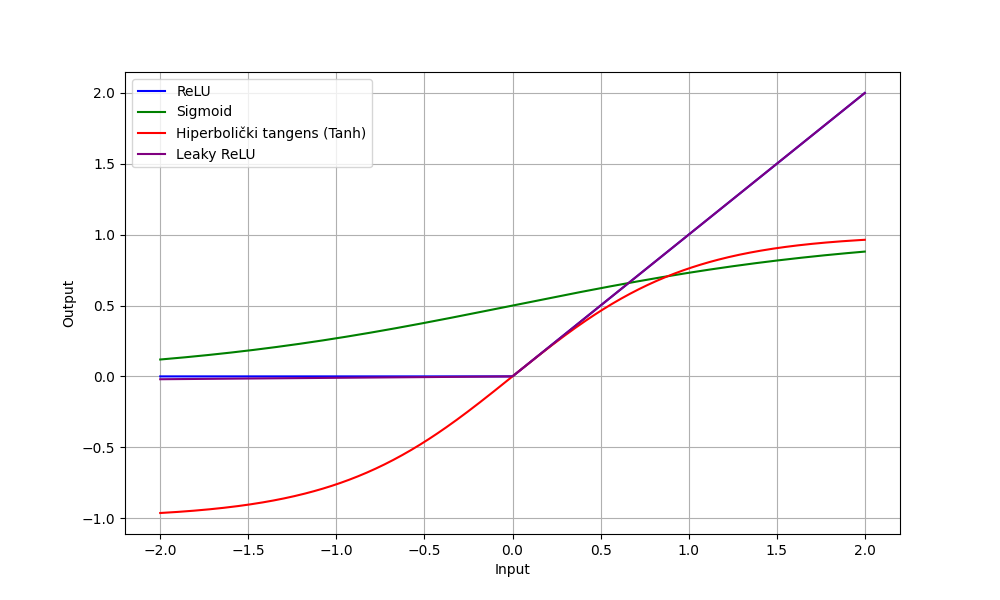
\includegraphics{pop_activations.png}} % Adjust the scale factor as needed
      \caption{Grafik najčešće korišćenih aktivacionih funkcija}
      \label{fig:pop_activations}
    \end{figure}

    \newpage 
    
    \subsection*{Pooling slojevi}
   Pooling slojevi su još jedna ključna komponenta \textbf{CNN}-ova koja vrši operaciju uzorkovanja po određenoj strategiji kako bi 
   se smanjile prostorne dimenzije ulazne \textit{feature} mape, čime se smanjuje 
   računarska složenost i sprečava prekomerno prilagođavanje (engl. \textit{overfitting}). 
   Najčešće korišćene operacije pooling-a su \textbf{\textit{max pooling}} i \textbf{\textit{average pooling}}.
   \subsubsection*{Pooling operacija}
   \textit{Pooling} operacije se primenjuju na svaku \textit{feature} mapu nezavisno. 
   Ulazna \textit{feature} mapa \( F \) ima dimenzije \( H \times W \), gde je \( H \) visina, 
   a \( W \) širina. \textit{Pooling} operacija pomera prozor veličine \( f \times f \) preko \textit{feature} mape
   , sa korakom \( s \).

   \subsubsection*{Max Pooling}

   Kod \textit{max pooling}-a, izlazna vrednost za svaki prozor je maksimalna vrednost 
   unutar tog prozora. Matematički, za \textit{feature} mapu \( F \) i \textit{pooling} prozor 
   veličine \( f \times f \) sa korakom \( s \), 
   operacija \textit{max pooling}-a se može izraziti kao:

   \[
   M(i, j) = \max_{0 \leq m < f, 0 \leq n < f} F(s \cdot i + m, s \cdot j + n)
   \]

   gde \( M(i, j) \) predstavlja vrednost izlazne \textit{feature} mape na poziciji \((i, j)\).

   \subsubsection*{Average Pooling}

   Kod \textit{average pooling}-a, izlazna vrednost za svaki prozor je prosečna vrednost unutar tog 
   prozora. Matematički, za \textit{feature} mapu \( F \) i \textit{pooling} prozor veličine 
   \( f \times f \) sa korakom \( s \), 
   operacija \textit{average pooling}-a se može izraziti kao:

   \[
   A(i, j) = \frac{1}{f^2} \sum_{m=0}^{f-1} \sum_{n=0}^{f-1} F(s \cdot i + m, s \cdot j + n)
   \]

   gde \( A(i, j) \) predstavlja vrednost izlazne mape karakteristika na poziciji \((i, j)\).

   
   \begin{figure}[h!]
      \centering
      \adjustbox{scale=0.7,center}{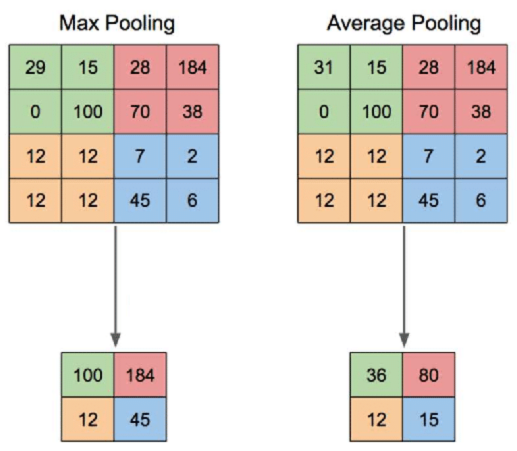
\includegraphics{pooling.png}} % Adjust the scale factor as needed
      \caption{Primer izvođenja \textit{max pooling} i \textit{average pooling} operacije}
      \label{fig:max_avg_pooling}
    \end{figure}

   \subsubsection*{Izlaz Pooling-a}

   Dimenzije izlazne \textit{feature} mape zavise od veličine prozora za pooling \( f \) i koraka \( s \). 
   Data ulazna \textit{feature} mapa \( F \) sa dimenzijama \( H \times W \), izlazna \textit{feature} mapa \( O \) 
   (bilo \( M \) za \textit{max pooling} ili \( A \) za \textit{average pooling}) ima dimenzije:
   
   \[
   H_{\text{out}} = \frac{H - f}{s} + 1
   \]
   \[
   W_{\text{out}} = \frac{W - f}{s} + 1
   \]
   
   gde su \( H_{\text{out}} \) i \( W_{\text{out}} \) visina i širina izlazne \textit{feature} mape, respektivno.
   

   \subsection*{Višeslojni Perceptron (MLP)}
   \subsubsection*{Perceptron}
    \vspace{-0.5cm}
   Perceptron prima više ulaznih signala, primenjuje težine na njih, 
   sabira ih i prosleđuje rezultat kroz aktivacionu funkciju kako bi proizveo izlaz (\textit{slika 6}).
   
   Za dat ulazni vektor \(\mathbf{x} = [x_1, x_2, \ldots, x_n]\) i odgovarajuće težine 
   \(\mathbf{w} = [w_1, w_2, \ldots, w_n]\), perceptron računa ponderisanu sumu na sledeći način:
   
   \[
   z = \sum_{i=1}^{n} w_i x_i + b
   \]
   
   gde je \(b\) (\textit{bias}) slobodan član.
   
   Izlaz \(y\) se zatim dobija primenom aktivacione funkcije \(f(z)\). U našem primeru smo za
   aktivacionu funkciju koristili \textbf{ReLU} funkciju, koja se definiše na sledeći način:
   \[
      y = 
      \begin{cases}
         z & \text{ako } z > 0 \\
         0 & \text{inače}
      \end{cases}
      \]
      
      
      \begin{figure}[h!]
         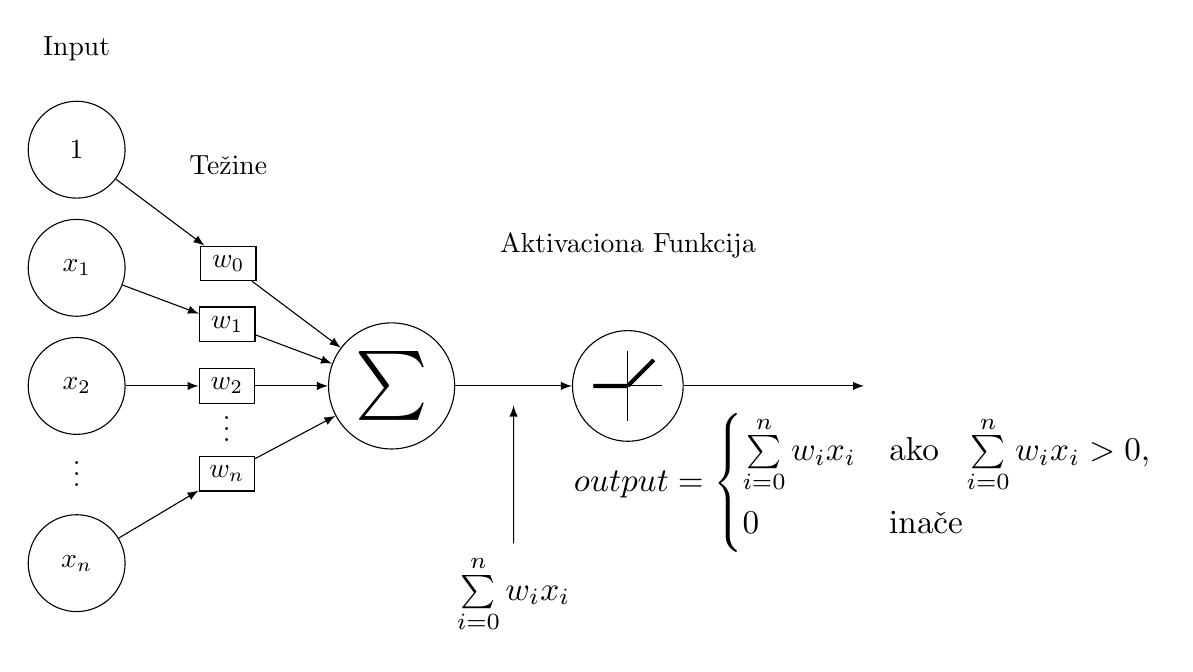
\begin{tikzpicture}[scale=1]
            
            % Draw input nodes
            \foreach \h [count=\hi ] in {$x_2$,$x_1$,$1$}{%
            \node[input] (f\hi) at (0,\hi*1.5cm-1.5 cm) {\h};
            }
            % Dot dot dot ... x_n
            \node[below=0.62cm] (idots) at (f1) {\vdots};
            \node[input, below=0.62cm] (last_input) at (idots) {$x_n$};
            % Draw summation node
            \node[functions] (sum) at (4,0) {\Huge$\sum$};
            % Draw edges from input nodes to summation node
            \foreach \h [count=\hi ] in {$w_2$,$w_1$,$w_0$}{%
            \path (f\hi) -- node[weights] (w\hi) {\h} (sum);
            \draw[->] (f\hi) -- (w\hi);
            \draw[->] (w\hi) -- (sum);
            }
         % Dot dot dot ... w_n
         \node[below=0.05cm] (wdots) at (w1) {\vdots};
         \node[weights, below=0.45cm] (last_weight) at (wdots) {$w_n$};
         % Add edges for last node and last weight etc
         \path[draw,->] (last_input) -- (last_weight);
         \path[draw,->] (last_weight) -- (sum);
         % Draw node for activation function
         \node[functions] (activation) at (7,0) {};
         % Place activation function in its node
         \begin{scope}[xshift=7cm,scale=1.25]
            \addaxes
            % flexible selection of activation function
            \relu
            %  \stepfunc
         \end{scope}
         % Connect sum to activation function
         \draw[->] (sum) -- (activation) node (sum_eq) [midway, below=2cm, scale=1.2] {$\sum\limits_{i=0}^n w_ix_i$} node (sum_activation_midway) [midway, below] {};
         \path[draw,->] (sum_eq) -- (sum_activation_midway);
         \draw[->] (activation) -- ++(3,0) node (perceptron_output) [below=0.2cm, scale=1.2] {$output = \begin{cases}\sum\limits_{i=0}^n w_ix_i & \text{ako }\ \sum\limits_{i=0}^n w_ix_i > 0,\\0 & \text{inače}\end{cases}$};
         % Labels
         \node[above=1cm]  at (f3) {Input};
         \node[above=1cm] at (w3) {Težine};
         \node[above=1.5cm] at (activation) {Aktivaciona Funkcija};
      \end{tikzpicture}
      \caption{Grafički prikaz perceptrona}
      \label{fig:perceptron}
   \end{figure}
   
   \subsubsection*{Višeslojni Perceptron (MLP)}
   \textbf{MLP} je potpuno povezana veštačka neuronska mreža koja se sastoji od više 
   slojeva perceptrona, obično uključujući ulazni sloj, jedan ili više skrivenih slojeva i 
   izlazni sloj.

   Za \textbf{MLP} sa \(L\) slojeva, ulaz u mrežu je \(\mathbf{x} \in \mathbb{R}^n\). 
   Izlaz svakog sloja \(l\) se računa kao:
   \[
   \mathbf{h}^{(l)} = f(\mathbf{W}^{(l)} \mathbf{h}^{(l-1)} + \mathbf{b}^{(l)})
   \]
   gde:
   \vspace{-0.5cm}
   \begin{itemize}
      \item \(\mathbf{h}^{(0)} = \mathbf{x}\) je ulazni vektor,
      \item\(\mathbf{W}^{(l)}\) i \(\mathbf{b}^{(l)}\) su matrica težina i vektor pristrasnosti za sloj \(l\),
      \item \(f\) je aktivaciona funkcija (obično \textit{ReLU}, \textit{sigmoid} ili \textit{tanh}).
   \end{itemize}

   Finalni sloj često koristi \textit{softmax} funkciju za klasifikacione zadatke, koja pretvara 
   izlaz u distribuciju verovatnoće za date klase:

   \[
   \text{softmax}(\mathbf{z})_i = \frac{e^{z_i}}{\sum_{j=1}^P e^{z_j}}
   \]

   gde je \(\mathbf{z}\) ulaz u softmax funkciju, a \(P\) je broj klasa.
   \vspace{0.5cm}

   \begin{figure}[h!]
      % NEURAL NETWORK with coefficients, uniform arrows
      \newcommand\setAngles[3]{
         \pgfmathanglebetweenpoints{\pgfpointanchor{#2}{center}}{\pgfpointanchor{#1}{center}}
         \pgfmathsetmacro\angmin{\pgfmathresult}
         \pgfmathanglebetweenpoints{\pgfpointanchor{#2}{center}}{\pgfpointanchor{#3}{center}}
         \pgfmathsetmacro\angmax{\pgfmathresult}
         \pgfmathsetmacro\dang{\angmax-\angmin}
         \pgfmathsetmacro\dang{\dang<0?\dang+360:\dang}
         }
      \centering
      \begin{tikzpicture}[x=3.2cm,y=1cm]
      \message{^^JNeural network with uniform arrows}
      \readlist\Nnod{4,5,3} % array of number of nodes per layer
      
      \foreachitem \N \in \Nnod{ % loop over layers
         \def\lay{\Ncnt} % alias of index of current layer
         \pgfmathsetmacro\prev{int(\Ncnt-1)} % number of previous layer
         \message{^^J Layer \lay, N=\N, prev=\prev ->}
         
         % NODES
         \foreach \i [evaluate={\y=\N/2-\i; \x=\lay; \n=\nstyle; \notation=(\lay==1)?"x":((\lay==\Nnodlen)?"y":"h");}] in {1,...,\N}{ % loop over nodes
               \message{N\lay-\i, }
               \node[node \n] (N\lay-\i) at (\x,\y) {$\notation_\i^{(\prev)}$};
            }    
         % CONNECTIONS
         \foreach \i in {1,...,\N}{ % loop over nodes
            \ifnum\lay>1 % connect to previous layer
            \setAngles{N\prev-1}{N\lay-\i}{N\prev-\Nnod[\prev]} % angles in current node
            %\draw[red,thick] (N\lay-\i)++(\angmin:0.2) --++ (\angmin:-0.5) node[right,scale=0.5] {\dang};
            %\draw[blue,thick] (N\lay-\i)++(\angmax:0.2) --++ (\angmax:-0.5) node[right,scale=0.5] {\angmin, \angmax};
            \foreach \j [evaluate={\ang=\angmin+\dang*(\j-1)/(\Nnod[\prev]-1);}] %-180+(\angmax-\angmin)*\j/\Nnod[\prev]
                        in {1,...,\Nnod[\prev]}{ % loop over nodes in previous layer
               \setAngles{N\lay-1}{N\prev-\j}{N\lay-\N} % angles out from previous node
               \pgfmathsetmacro\angout{\angmin+(\dang-360)*(\i-1)/(\N-1)} % number of previous layer
               %\draw[connect arrow,white,line width=1.1] (N\prev-\j.{\angout}) -- (N\lay-\i.{\ang});
               \draw[connect arrow] (N\prev-\j.{\angout}) -- (N\lay-\i.{\ang}); % connect arrows uniformly
            }
            \fi % else: nothing to connect first layer
         }
      }
      
      % LABELS
      \node[above=5,align=center,mygreen!60!black] at (N1-1.90) {input\\[-0.2em]sloj};
      \node[above=1,align=center,myblue!60!black] at (N2-1.90) {skriveni slojevi};
      \node[above=8,align=center,myred!60!black] at (N\Nnodlen-1.90) {output\\[-0.2em]sloj};
      
      \end{tikzpicture}
      \caption{Grafički prikaz \textbf{MLP}-a sa 4 ulazna, 5 skrivenih i 3 izlazna čvora}
      \label{fig:mlp}
   \end{figure}

   \newpage
   \section{Transformeri}
   \subsection{Istorija i razvoj}
   Model \textbf{Transformera}, predstavljen u seminalnom radu \textit{"Attention is All You Need"} \cite{attentionneed} od Vaswani-ja i saradnika 2017. godine, 
   označio je značajan napredak u oblasti obrade prirodnog jezika (\textbf{NLP}). 
   Pre toga, modeli kao što su \textit{Recurrent Neural Networks} (\textbf{RNNs}) \cite{rnn} i 
   \textit{Long Short-Term Memory Networks} (\textbf{LSTMs}) \cite{lstm} bili su dominantne arhitekture za 
   \textit{sequence-to-sequence} zadatke. Međutim, ovi modeli su imali ograničenja, 
   posebno sa udaljenim zavisnostima i paralelizacijom.

   Transformeri su revolucionisali \textbf{NLP} uvođenjem nove arhitekture koja se u potpunosti zasniva na 
   \textbf{\textit{self-attention}} mehanizmu, eliminišući potrebu za rekurentnim slojevima. 
   Ova inovacija je omogućila efikasnije treniranje i sposobnost da se bolje modeluju veze između 
   udaljenih reči u sekvenci. Uvođenje transformera dovelo je do dramatičnog poboljšanja performansi 
   na različitim \textbf{NLP} zadacima, kao što su mašinsko prevođenje, sažimanje teksta i odgovaranje na pitanja.

   Njihov uspeh brzo je postao evidentan razvojem moćnih modela koji su ih koristili kao osnovu. 
   Jedna od prvih značajnih primena bila je u mašinskom prevođenju, gde je transformer 
   nadmašio prethodne najbolje modele na referentnim skupovima podataka. 
   Ovaj uspeh je dodatno pojačan stvaranjem modela kao što su \textbf{BERT} 
   \textit{(Bidirectional Encoder Representations from Transformers)} \cite{bert} i \textbf{GPT} 
   \textit{(Generative Pre-trained Transformer)} \cite{gpt2}, koji su postavili nove standarde za 
   različite \textbf{NLP} zadatke.

   \newpage   
   \printbibliography[title={Reference}]
\end{document}